\section{Applikationssicherheit}
\label{sec:security}

\subsection{Zeitsynchronisierung}
\label{subsec:timesync}

In diesem Abschnitt werden Probleme besprochen, die durch fehlerhafte respektive
mangelhaft durchdachte Zeitsynchronisierung oder Verbindungsabbruch entstehen
können.

\paragraph{Problem durch falsche Zeitstempel bei Logeinträgen:}
Betrachtet wird das Szenario ``Umladevorgang eines Produktes''. Das mobile
Gerät der Transporteinheit wird benutzt um den Ausladevorgang aus einem
Container im System zu verarbeiten. Mit dem scannen des Produkts wird auf dem
mobilen Gerät der Transporteinheit ein Logeintrag in dessen lokale Datenbank
erstellt. Genauso wird beim darauffolgenden Ladevorgang der Umladestation ein
Logeintrag auf dessen Gerät erstellt. Wenn das System mit absoluter Zeit
arbeitet und die Uhrzeit des Geräts der Transporteinheit vor jener der
Umladestation ist, dann würde im System der Übernahmevorgang der Umladestation
vor dem Ausladevorgang der Transporteinheit stattfinden.
\par
\paragraph{Lösungsansatz:}
Um dieses Problem zu lösen muss relative Zeit eingeführt und synchronisiert
werden. Für die Zeitsynchronisierung können bekannte Algorithmen für verteilte
Systeme verwendet werden. Mögliche Algorithmen sind Christian's Algorithm oder Berkley Algorithm\footnote{$http://en.wikipedia.org/wiki/Clock_synchronization$}.
\par
Im Projekt Roadrunner wurde Christian's Algorithmus implementiert. Jeder Client misst seine Differenz zur Serverzeit und verwendet diese zur Erzeugung der Zeitstempel. Somit können die unterschiedlichen Uhren bis zu einer gewünschten Genauigkeit synchronisiert werden.

Grundsätzlicher Ablauf zur Ermittlung der Zeitdifferenz ist folgender:
\begin{enumerate}
\item Client erzeugt einen Zeitstempel mit der letzten bekannten Differenz zur Serverzeit.
\item Client sendet eine Anfrage für die Serverzeit an den Server.
\item Server antwortet mit seiner Zeit.
\item Client erzeugt einen zweiten Zeitstempel.
\item Ist die RoundTrip-Zeit klein genug werden die Zeitstempel von Client und Server verglichen.
\item Überschreitet die Zeitdifferenz einen Schwellwert wird auf dem Client die neue Zeitdifferenz gesetzt.
\end{enumerate}

\par
Die Uhren werden bis zu einer gewählten Genauigkeit miteinander synchronisiert. Beim Projekt Roadrunner wurde die Genauigkeit mit 5 Sekunden gewählt. Dies bedeutet, wenn der Client seinen Zeitstempel mit dem von dem Server vergleicht und die Differenz die Genauigkeit überschreitet, dann ermittelt der Client die neue Differenz und verwendet diese zur Erzeugung der nächsten Zeitstempel. Die Synchronisation bis zu einer Genauigkeit von 5 Sekunden wurde gewählt, da ein Umladevorgang sicher länger als 5 Sekunden dauert. Eine zu kleine Genauigkeit hätte zur Folge, dass durch Abweichende RoundTrip-Zeiten ständig die Uhr neu gestellt würde und unnötig viele Zeitsynchronisierungseinträge erstellt würden.
\par
Bei jeder Zeitsynchronisierung wird eine Log-Eintrag für alle geladenene Items erzeugt. Dadurch ist in der History eines Items ersichtlich wann eine Zeitsynchronisierung des Client durchgeführt wurde und welche Log-Einträge einen von der Serverzeit abweichenden Zeitstempel haben.
\par
Bei der Zeitsynchronisierung ist die RoundTrip-Zeit ebenfalls von großer Bedeutung. Ist die RoundTrip-Zeit zu groß wird der Zeitstempel vom Server verworfen und keine Synchronisierung durchgeführt. Nur wenn die RoundTrip-Zeit hinreichend klein ist, kann eine sinnvolle Zeitdifferenz der Zeitstempel ermittelt werden. Für die größte noch erlaubte RoundTrip-Zeit wurde 2 Sekunden gewählt. Dies entspricht etwa der halben Genauigkeit und bei keiner zu großen Netzauslastung sollte ein Request in dieser Zeit auch abarbeitbar sein.

\subsection{Zugriffskontrolle}

Zur Umsetzung des Rechtesystems von Roadrunner werden verschiedene Benutzergruppen eingeführt. Die Rechte werden einerseits direkt auf der Datenbank definiert und zudem noch über Validierungsfunktionen umgesetzt. Die Benutzerauthentifizierung wird von CouchDB durchgeführt.

\subsection{Administratoren \& Benutzer}

\begin{figure}
	\centering
		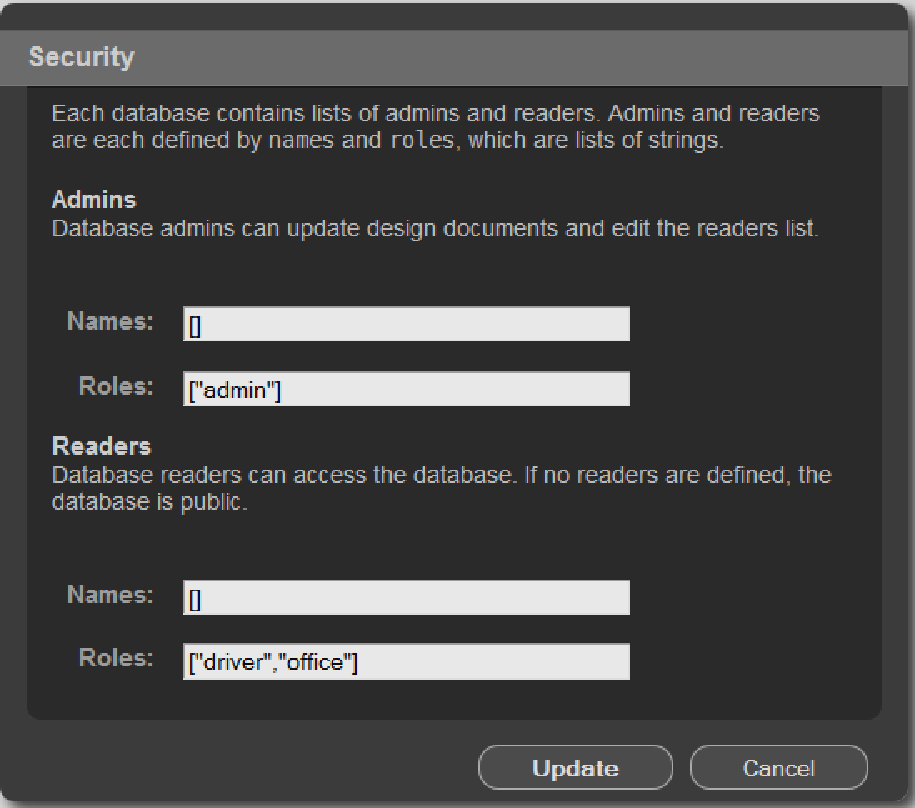
\includegraphics[width=0.8\textwidth]{files/pdf/security.pdf}
	\caption{Admins \& Readers}
	\label{fig:security}
\end{figure}

Auf einer Datenbank können in CouchDB Admins und Readers definiert werden. 
\begin{description}
\item[Admin] Ein Admin hat sämtliche Rechte auf der Datenbank. Er kann die zudem die Datenbank löschen, Designdokumente verändern oder Benutzerrechte ändern.
\item[Reader] Ein Reader hat lesenden und schreibenden Zugriff auf alle Dokumente bis auf die Designdokumente.
\end{description}

\noindent Ein Benutzer kann über 2 verschiedene Arten einer Gruppe zugeordnet werden:
 \begin{itemize}
\item Names: Ein CouchDB-Benutzer muss einen eindeutigen Namen im Format "`org.couchdb.user:[username]"' haben. Die Benutzer werden in einer seperaten Datenbank mit dem Namen "`\_users"' definiert. Wenn der Benutzer dieser Liste (Array aus Strings) hinzugefügt wird, dann besitzt er die entsprechenden Rechte.
\item Roles: Ein Benutzer kann verschiedene Rollen besitzen. Wenn eine seiner Rollen in dieser Liste aufgeführt wird, hat er die entsprechenden Rechte. 
\end{itemize}

\subsubsection{Rollen in Roadrunner}

Einem Benutzer können keine bis mehrere Rollen zugewiesen werden. Bei jeder Veränderung von Dokumenten auf dem Backendsystem wird von CouchDB eine Benutzerauthentifizierung durchgeführt. Bei dieser Benutzerauthentifizierung wird das Zugriffsrecht auf die Datenbank überprüft und zudem eine Validierung durchgeführt. Bei der Validierung werden alle definierten Validierungsmethoden aufgerufen. Nur wenn alle Validierungen gültig sind wird die gewünschte Änderung an den Dokumenten durchgeführt.
\newline \newline \noindent
Im Projekt Roadrunner wurden 3 verschiedenen Rollen definiert:
\begin{description}
\item[Admin] Ein Admin hat sämtliche Rechte auf der Datenbank. Diese Rollen ist ausschließlich für Administratoren vorgesehen.
\item[Office] Ein Benutzer der Gruppe Office arbeitet mit dem Backendsystem von Roadrunner. Dieser Benutzer arbeitet über die Webapplikation mit Roadrunner.
\item[Driver] Ein Benutzer der Gruppe Driver ist ein Fahrer. Er arbeitet auf dem Androidsystem mit Roadrunner. Auf dem Androidsystem arbeitet er als Admin mit der Datenbank. Eine Einschränkung der Benutzerrechte auf dem Androidsystem ist nicht nötig da die Benutzerauthentifizierung bei der Replizierung der Daten von dem Androidsystem auf das Backendsystem durchgeführt wird. Ein Fahrer kann nur Daten replizieren für die er die entsprechenden Rechte besitzt.
\end{description}

\noindent In den Validierungsmethoden werden die entpsrechenden Rechtevalidierungen durchgeführt. In Tabelle \ref{tab:rechte} sind die Berechtigungen aufgelistet. Ein + bedeutet, dass der Benutzer das Recht besitzt.

\begin{table}
\begin{tabular}{lccc}
	& Driver & Office & Admin \\
	Benutzerrechte ändern & - & - & + \\
	Designdokumente ändern & - & - & + \\
	Logeinträge anlegen & + & + & + \\
	Logeinträge ändern & - & - & + \\
	Logeinträge löschen & - & - & + \\
	Andere Dokumente anlegen & - & + & + \\
	Andere Dokumente ändern & - & + & + \\
	Andere Dokumente löschen & - & + & +
\end{tabular}
\caption{Benutzerrechte}
\label{tab:rechte}
\end{table}
